%===================================== CHAP 3 =================================

\chapter{Results}

For this project, the pressure and blood flow velocities of seven patients were recorded. For each patient, four recordings taken on separate stages of the disease were used in the analysis. As thoroughly discussed in the previous chapters, in the absence of disease, the cardiac systems of the body can locally adjust their vascular resistance and compliance to maintain adequate blood flow and cardiac output to critical organs. During severe sepsis or septic shock, it is believed that these autoregulatory properties fail at maintaining homeostasis in the cardiovascular system. Since both the SVR and compliance are the two main parameters of the cardiovascular model, one should be able to identify a pattern of autoregulation malfunction by observing the lower frequencies of these parameters.

The patients' state at any stage of the recordings was not revealed before the final week of the project, i.e., one week before the project report deadline. The intention was that without any preliminary knowledge of the patients' state, one should be able to recognize if the patient was getting worse or recovering from sepsis. 

The first section will follow the state and analysis of one patient, which will be referred to as patient 18. The following section will then show the results of multiple patients.



\section{Sepsis severity indicator}\label{sect:sepsis_severity}
The amount of Norepinephrine (NE), also called noradrenaline, given to the patient, along with the mean arterial pressure (MAP), can be used as a marker of the severity of sepsis. NE is used as a first-line agent in hypotensive patients affected by septic shock. NE is a vasopressor, which is a medicine that stabilizing blood perfusion by contracting (tightening) the blood vessels when the patient is suffering from extremely low blood pressure. \cite{RN20} The NE infusion is proportional to the severity of the shock, i.e., the dosage is increased if the condition of the patient is more critical. Patient 18 were given the following dose in chronological order of the recordings taken at different dates: 
\begin{itemize}
    \itemsep0em
    \item \textbf{19.01.2019}: 0.07 [micrograms/kg/min]
    \item \textbf{20.01.2019}: 0.12 [micrograms/kg/min]
    \item \textbf{21.01.2019}: 0.13 [micrograms/kg/min]
    \item \textbf{23.01.2019}: 0.11 [micrograms/kg/min]
\end{itemize}
From this, we can tell that patient 18's condition is better in the first recording, gets worse the next two days, and is less severe in the last recorded day as the patient responds to appropriate treatment.



\section{Patient 18}

This section will analyze the 2-element WK parameters in both time and frequency domain. First, the calculated parameters for each recording for the patient will be presented and examined, before a more in-depth investigation of their lower frequencies.


\subsection{2-element WK parameters}\label{sect:WKparameters}

The SVR and compliance were calculated for all four recordings according to the parameter extraction shown in the diagram in figure \ref{fig:parameter_diagram} in section \ref{sect:parameter_estimation}. For patient 18, we saw a small spike in the NE dose from 19.01 to 20.01, which was then slightly reduced again in the last recording as the patient most likely responded to treatment. Before analyzing any deeper, it should be mentioned that the parameter values are converted to a relative, comparable, and unitless scale by dividing by the mean parameter value. The reason being that all the measurements with larger value ranges oscillated with much more magnitude relative to the others, which would make them outweigh the others in both time and frequency domain. From the SVR in figure \ref{fig:resistance_patient18}, you can see the state of the patient get worse from the top plot of the figures until the second to last, by the parameter's stochasticity. For the compliance, however, it seems like the severity is worst in the first recording, and dampens off in the subsequent measurements. These kinds of discrepancies will be further discussed in the next chapter.

\begin{figure}[h!]
    \centering
    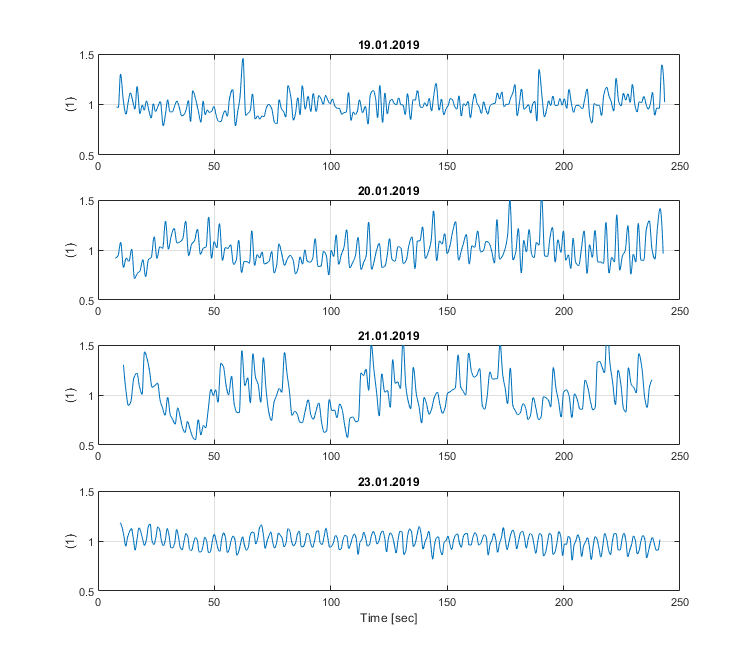
\includegraphics[width=0.7\textwidth]{fig/results/resistance_patient18_rel.png}
    \caption{SVR of patient 18 calculated from 4 different recordings. Since each parameter measurement had different ranges and offsets, each of the measurements are divided by their own mean to convert them to a unitless and comparable scale.}
    \label{fig:resistance_patient18}
\end{figure}{}

\begin{figure}[h!]
    \centering
    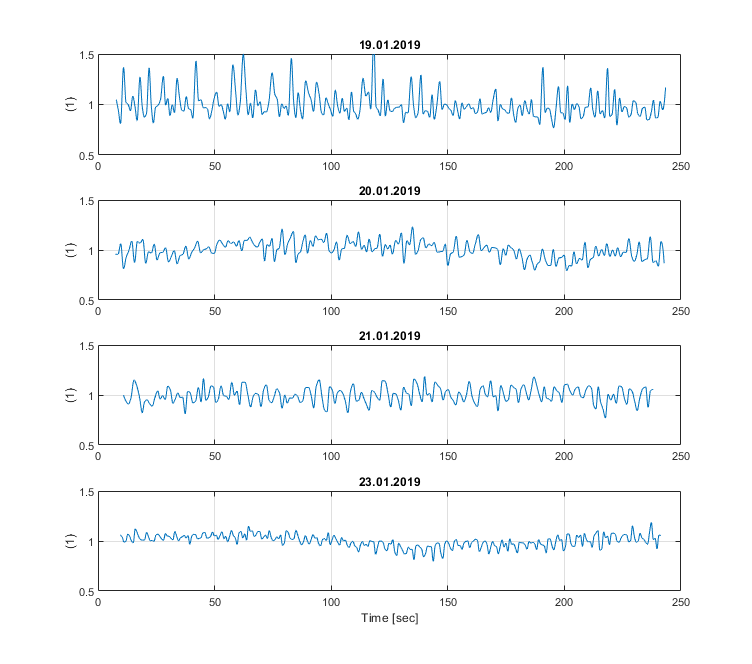
\includegraphics[width=0.7\textwidth]{fig/results/compliance_patient18_rel.png}
    \caption{The arterial compliance of patient 18 calculated from 4 different recordings.}
    \label{fig:compliance_patient18}
\end{figure}{}

\newpage

\subsection{Parameter frequency analysis}

The frequency spectrum of the resistance is shown in figure \ref{fig:resistance_dft} and compliance in figure \ref{fig:compliance_dft}. The magnitude of the frequency components has been converted to a comparable, unitless scale. In the left plot of both figures shows the magnitude of the frequency band 0.0085-0.0382 Hz (20-120 second oscillations) for each recording. From the frequency spectrum of the resistance in figure \ref{fig:resistance_dft_magnitude}, you can see the large contribution from the 40-80 second variations in the parameters. This is even more evident in the next plot in figure \ref{fig:resistance_dft_mean_magnitude}, which shows the average magnitude of the whole frequency band, as well as the NE dosage given to the patient at the different dates of the recordings. The resistance seems to follow the state of the patient given by the increased dosage of NE. The compliance, however, seems to show a decreasing trend in the magnitude following the increased dosage if NE, which conforms with the analysis in the previous section.

\begin{figure}[h]
  \centering
      \subfloat[magnitude of the \textit{slow} variations in resistance ($\sim$20-125 seconds).]{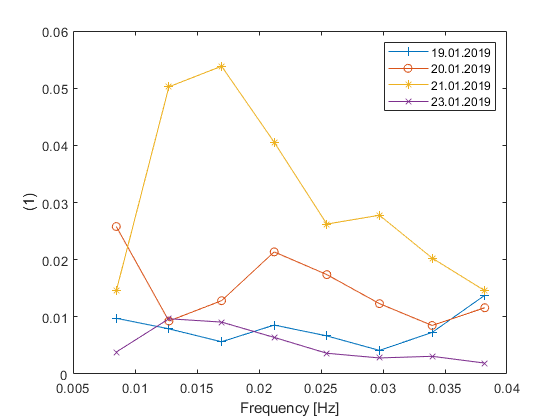
\includegraphics[width=0.48\textwidth]{fig/results/resistance_dft_magnitude.png}
      \label{fig:resistance_dft_magnitude}}
      \hfill
      \subfloat[Mean magnitude of the frequencies shown in (a).]{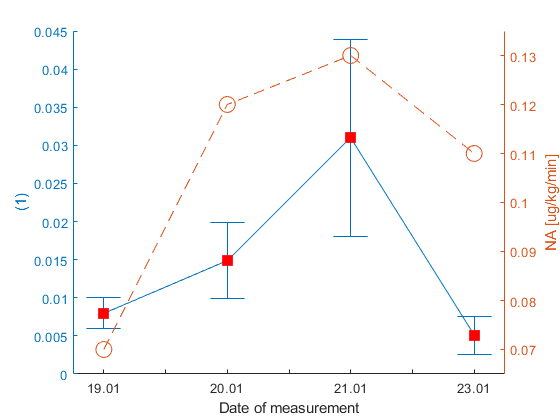
\includegraphics[width=0.48\textwidth]{fig/results/resistance_dft_mean_magnitude.png}
      \label{fig:resistance_dft_mean_magnitude}}
  \caption{The frequency analysis of the SVR of all recordings. The experimental theory is that the lower frequencies of the parameter, which will manifest itself as low-frequency noise and increase the average magnitude. Figure (b) shows the mean value of each recording of the frequency spectrum in (a).}
  \label{fig:resistance_dft}
\end{figure}


\begin{figure}[h]
  \centering
      \subfloat[magnitude of the \textit{slow} variations in resistance ($\sim$20-125 seconds).]{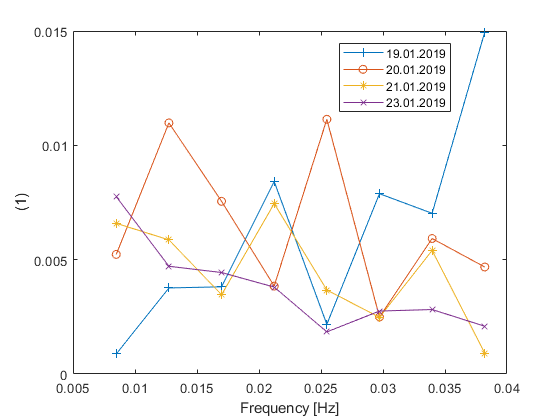
\includegraphics[width=0.48\textwidth]{fig/results/compliance_dft_magnitude.png}
      \label{fig:compliance_dft_magnitude}}
      \hfill
      \subfloat[Mean magnitude of the frequencies shown in (a).]{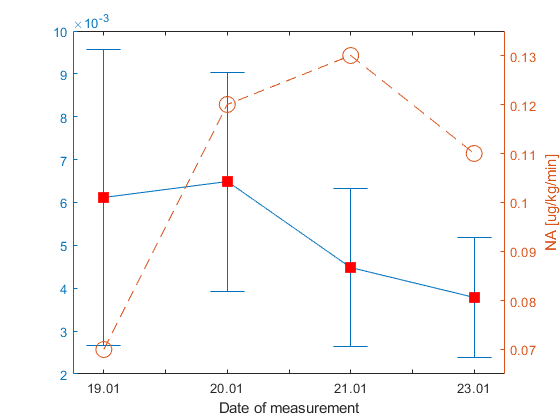
\includegraphics[width=0.48\textwidth]{fig/results/compliance_dft_mean_magnitude.png}
      \label{fig:compliance_dft_mean_magnitude}}
  \caption{The frequency analysis of the arterial compliance of all recordings. The experimental theory is that the lower frequencies of the parameter, which will manifest itself as low-frequency noise and increase the average magnitude. Figure (b) shows the mean value of each recording of the frequency spectrum in (a).}
  \label{fig:compliance_dft}
\end{figure}

\newpage

\section{All patients}

Figure \ref{fig:resistance_dft_all} and \ref{fig:compliance_dft_all} respectively shows the resistance and compliance of all the available patients with usable blood pressure and velocity measurements. They both show the mean magnitude of the frequencies within the band of interest, the same way it was presented in the r.h.s. plot of the figures from the previous section. There seems to a bit hard to correlate the average magnitude of the lower frequency band and the state of the patient, given the NE dosage. The relationship between the NE dose and the state of the patient is not always correct; some patients can either get better by themselves, respond to the treatment, or a combination of the two. It is fair to say, however, that the majority of the results seem to follow the hypothesis that there either is a larger average magnitude in the frequency band of interest corresponding with a greater NA dosage.

\begin{figure}[h]
    \centering
    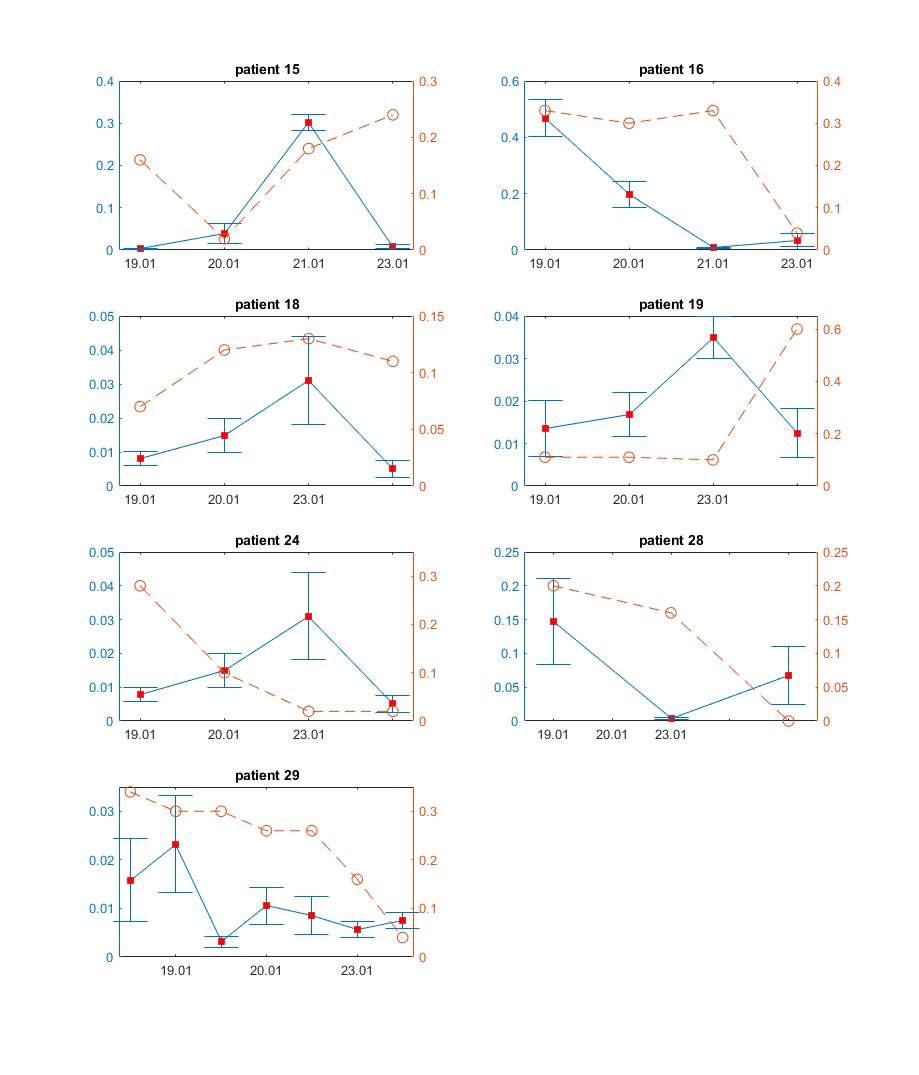
\includegraphics[width=1\textwidth]{fig/results/resistance_dft_all.png}
    \caption{Mean SVR magnitude within the frequency band of interest for all patients.}
    \label{fig:resistance_dft_all}
\end{figure}{}

\begin{figure}[h]
    \centering
    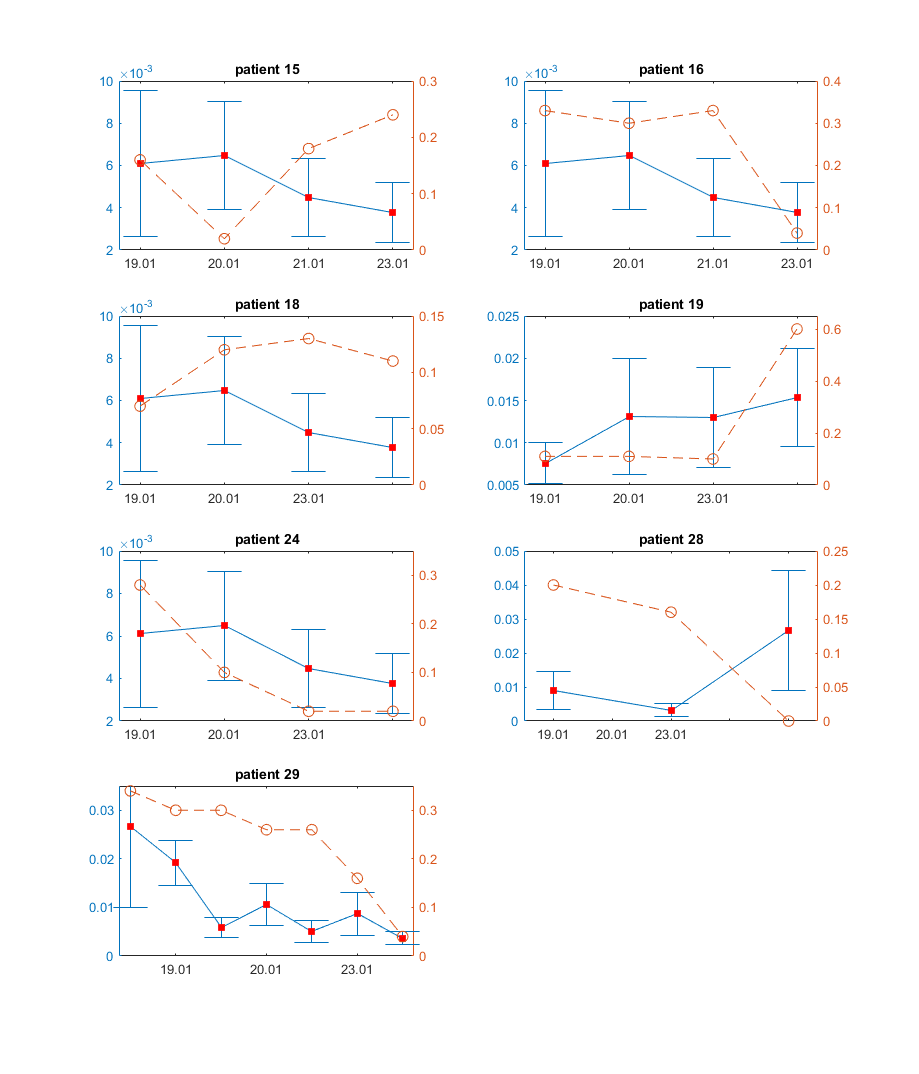
\includegraphics[width=1\textwidth]{fig/results/compliance_dft_all.png}
    \caption{Mean compliance magnitude within the frequency band of interest for all patients.}
    \label{fig:compliance_dft_all}
\end{figure}{}

\cleardoublepage